% Correct rate before (open circle) and after (filled circle) each A/B comparison that reports one.
% x = percent * 0.085 cm; the label column is 5.2 cm wide.
\begin{figure}[htbp]
\centering
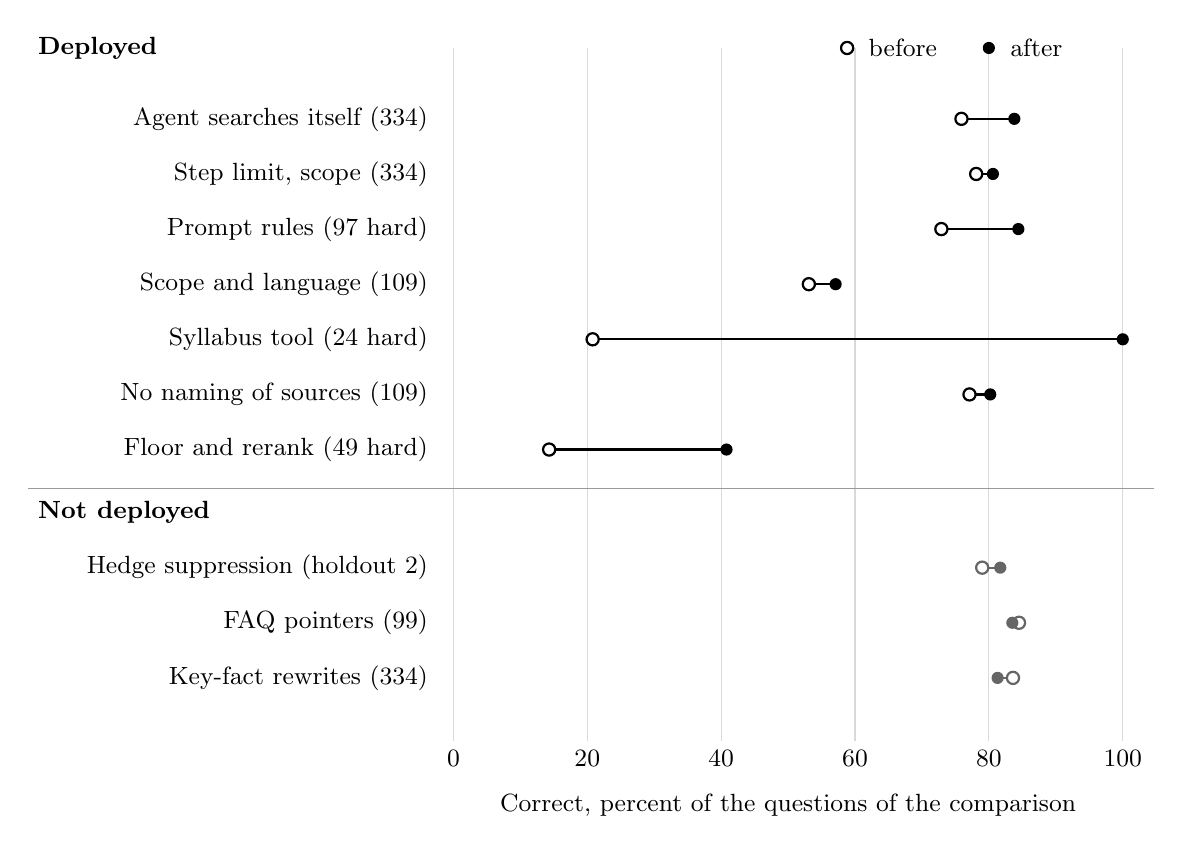
\begin{tikzpicture}[x=1cm,y=1cm,font=\small]
  \foreach \p in {0,20,40,60,80,100} {
    \draw[black!15] ({0.085*\p},0.5) -- ({0.085*\p},-8.3);
    \node[below] at ({0.085*\p},-8.3) {\p};
  }
  \node[below] at (4.25,-8.85) {Correct, percent of the questions of the comparison};
  \node[anchor=west] at (-5.4,0.5) {\textbf{Deployed}};
  \foreach \y/\lab/\b/\a in {
      -0.4/{Agent searches itself (334)}/75.9/83.8,
      -1.1/{Step limit, scope (334)}/78.1/80.6,
      -1.8/{Prompt rules (97 hard)}/72.9/84.4,
      -2.5/{Scope and language (109)}/53.1/57.1,
      -3.2/{Syllabus tool (24 hard)}/20.8/100,
      -3.9/{No naming of sources (109)}/77.1/80.2,
      -4.6/{Floor and rerank (49 hard)}/14.3/40.8} {
    \node[left,align=right] at (-0.2,\y) {\lab};
    \draw[black,line width=.8pt] ({0.085*\b},\y) -- ({0.085*\a},\y);
    \fill[white,draw=black,line width=.8pt] ({0.085*\b},\y) circle (2.2pt);
    \fill[black] ({0.085*\a},\y) circle (2.2pt);
  }
  \draw[black!40] (-5.4,-5.1) -- (8.9,-5.1);
  \node[anchor=west] at (-5.4,-5.4) {\textbf{Not deployed}};
  \foreach \y/\lab/\b/\a in {
      -6.1/{Hedge suppression (holdout 2)}/79.0/81.7,
      -6.8/{FAQ pointers (99)}/84.5/83.5,
      -7.5/{Key-fact rewrites (334)}/83.6/81.3} {
    \node[left,align=right] at (-0.2,\y) {\lab};
    \draw[black!60,line width=.8pt] ({0.085*\b},\y) -- ({0.085*\a},\y);
    \fill[white,draw=black!60,line width=.8pt] ({0.085*\b},\y) circle (2.2pt);
    \fill[black!60] ({0.085*\a},\y) circle (2.2pt);
  }
  % legend
  \fill[white,draw=black,line width=.8pt] (5.0,0.5) circle (2.2pt);
  \node[right] at (5.15,0.5) {before};
  \fill[black] (6.8,0.5) circle (2.2pt);
  \node[right] at (6.95,0.5) {after};
\end{tikzpicture}
\caption[Correct rate before and after each change of the live system, for the comparisons that report one (set size in brackets)]{Correct rate before and after each change of the live system, for the comparisons that report one (set size in brackets). Table~\ref{tab:live-ab} explains each change in one line. Open circles show the baseline and filled circles the changed configuration. ``Hard'' sets contain emails that earlier runs answered wrongly, so their baseline is low and their gains are inflated. The first row is derived from counts (7 and 20 of 49). Rejected or not deployed changes are in grey. Comparisons that report other measures (refusals, empty lookups, broken links, hedge phrases) appear only in the table in Appendix~\ref{app:live}.}
\label{fig:live-ab}
\end{figure}
